\graphicspath{{bundles/}}


\chapter{The Trajectory Bundle Method}
\label{sec:bundles}
We present a derivative-free trajectory optimization technique that approximates functions with linear interpolation between samples instead of using a Taylor series. The resulting algorithm, the trajectory bundle method, is able to exploit accelerators to compute parallelized samples of the cost, dynamics, and constraint functions to form the linear interpolants. These so-called bundles are then used in a convex optimization problem that is solved for the next iterates within a trust region. This process is repeated until tight constraint satisfaction is achieved, and is a significant improvement over existing derivative-free optimization techniques when applied to trajectory optimization problems. The efficacy of this method is demonstrated on a variety of robotics platforms.


\section{Introduction}\label{sec:bundles:introduction}
Linear dynamical systems of the form $x_{+} = Ax + Bu$ underpin many of the foundational methods in modern optimal control. Ideas like the Linear Quadratic Regulator (LQR) and convex trajectory optimization are able to reason about dynamical systems of this form in a way that is exact and globally optimal \cite{kalman1960,borrelli2017,boyd2004}. As a result, these techniques are often applied to nonlinear systems where a locally approximate linear dynamical system is used instead of the nonlinear model in a process called linearization \cite{slotine1991}. In many cases, this approximation is appropriate given this approximation is not used too far outside of the linearization point where the approximation was formed. By being careful about where these approximations are initialized and how far from their linearization point they are being used, this method of linearizing nonlinear systems can be extremely effective in practice, even for highly nonlinear systems.  The two caveats here are that the nonlinear system must be both smooth and differentiable. 

For many systems such as robotic arms, quadrotors, and vehicles, this assumption of smooth differentiability is appropriate. For rigid-body dynamics, there are specialized methods for computing derivatives through the continuous-time dynamics in a fast and efficient way \cite{featherstone1987}. However, there are also scenarios where these derivatives are either unavailable, prohibitively expensive to compute, or are unreliable. If the dynamics model is learned from data, the approximation of the dynamics function may be good while the approximation of the derivatives may be very poor. This scenario is often explored in the context of model-predictive path-integral control, where a learned simulator is only used to produce parallelized rollouts \cite{williams2016, wagener2019}. Another scenario in which derivatives are unavailable or unusable is in the presence of systems that make or break contact. While there has been a lot of recent interest in making simulations with contact differentiable \cite{freeman2021, newbury2024, pang2023, tracy2023b, suh2022a, howell2022}, there remains a strong need for optimal control methods that do not rely on these derivatives at all.  

A prevalent trend in robotic simulation is the introduction of simulators that can be run on accelerators for massively parallel simulation. Popular simulators like Isaac Sim \cite{makoviychuk2021, mittal2023}, Brax \cite{freeman2021}, and MuJoCo XLA (MJX) \cite{todorov2012}, are all capable of running thousands of simulations in parallel. This paper looks to leverage the innovation of parallel simulation to motivate a new optimal control paradigm where derivative-free simulations are used to describe the dynamics and cost landscapes present in the problem. To this effect, we present the trajectory bundle method for solving nonconvex trajectory optimization problems in an entirely derivative-free manner. This method uses interpolated short simulations instead of derivative-based linearization to approximate the cost, dynamics, and constraint functions in the problem. The result is a simple and efficient trajectory optimization solver that can fully utilize parallelized simulation without requiring any derivatives. 

Derivative-Free Optimization (DFO) is a well-studied technique for solving optimization problems where derivatives are unavailable for whatever reason. John Dennis gives an appropriate description of motivation for DFO problem in \cite{powell1994} as to ``find the deepest point of a muddy lake,
given a boat and a plumb line, when there is a price to be paid for each sounding''. With modern accelerators capable of massively parallel dynamics, cost, and constraint evaluation, there is still a price to take soundings, but no longer a price \textit{for each} sounding.   In a seminal 1965 paper, the Nelder-Mead method for derivative-free function minimization was proposed where a simplex of sample points is used to approximate the cost landscape instead of derivatives. Methods like Mesh Adaptive Direct Search (MADS) \cite{audet2006} and NOMAD \cite{ledigabel2011, audet2021} followed, with improvements to the Nelder-Mead method. 

Although there has been much work on general DFO \cite{conn1997, kochenderfer2019,conn2009}, there are two notably similar approaches to the trajectory bundle method. The first is the Constrained Optimization by Linear Interpolation (COBYLA) solver, where the cost and constraint functions are approximated with linear interpolation \cite{powell1994}, and \cite{cartis2019}, where a residual cost function structure is assumed and samples are used for linear interpolation. The trajectory bundle method builds on these two methods and specializes to trajectory optimization problems where the decision variables are only coupled via the dynamics constraints. By exploiting this problem-specific structure and massively parallelizable simulation, the trajectory bundle method is  simple and robust method for solving trajectory optimization problems to tight constraint and optimality tolerances.


% \plan{
% \begin{itemize}
%     \item talk about how optimal control and trajectory optimization work on linear models
%     \item we extend these methods to deal with nonlinear systems by linearizing these models 
%     \item this is usually done with a first order taylor series 
%     \item there are many scenarios where these derivatives are hard to get, expensive to get, or are entirely meaningless 
%     \item in the meantime, the cost of parallel simulation is rapidly decreasing 
%     \item this work we propose a new method for trajectory optimization based on multiple shooting 
%     \item there are no derivatives required of anything, all we need is a black box simulator 
% \end{itemize}
% }
% Our specific contributions in this paper are the following:
% \begin{itemize}
%     \item A derivative-free method for constrained trajectory optimization
%     \item An extension of this method to batch state estimation problems
% \end{itemize}


% citations:

% \begin{itemize}
%     \item original nelder mead \cite{nelder1965}
%     \item closest example from powell (direct search opt by linear interp) \cite{powell1994}
%     \item recent progress in unconstarined opt without derivatives \cite{conn1997}
%     \item mesh adaptive search for constrained \cite{audet2006}
%     \item textbook on derivative-free opti \cite{conn2009}
%     \item robust optimization with simulated annealing \cite{bertsimas2010}
%     \item NOMAD algorithm (which is really MADS alg) \cite{ledigabel2011}
%     \item sqp for derivative free optimization with equality cons \cite{troltzsch2016}
%     \item another textbook on blackbox opt \cite{audet2017}
%     \item mykels book \cite{kochenderfer2019}
%     \item another nomad reference \cite{audet2021}
%     \item evosax \cite{lange2022}
%     \item derivative-free gauss newton \cite{cartis2019}
% \end{itemize}




\section{Background}\label{sec:bundles:background}
Like many nonlinear optimization algorithms, the trajectory bundle method handles nonlinear cost and constraint functions by approximating them locally with affine functions. In this section, the standard method for approximating functions as affine with a Taylor series is detailed, followed by a derivative-free method using linear interpolation over sampled points.  Using these linear interpolants, the process for locally approximating a generic constrained optimization problem as convex is shown. 
%
%
\subsection{Affine Function Approximation}\label{btb:sect:interp}
%
%
% Nonlinear functions present a challenge for numerical optimization, where the nonlinearity often results in nonconvex optimization problems. For optimization problems where 



% In the context of numerical optimization, affine functions (both in the costs and constraints) are significantly easier to deal with than nonlinear ones. 
% This often means that it is adventageous to approximate an intractible nonlinear optimization problem with a locally-approximate 
An arbitrary function $p : \mathbf{R}^a \rightarrow \mathbf{R}^b$ is only affine if it can be represented in the following form: $p_\text{aff}(y) = d + Cy$, where $d \in \R{b}$ and $C \in \R{b \times a}$.
% Nonlinear functions can often be be approximated locally with an affine function through a variety of methods.
The process of locally approximating a nonlinear function with an affine function around a point $\bar{y}$ is often referred to as linearization, with $\bar{y}$ denoted as the linearization point. In this section, the standard method of approximation by first-order Taylor series is presented, followed by a derivative-free method involving linear interpolation of sample points.
% While these affine approximations are only accurate in some local neighborhood, the 
% Replacing nonlinear unctions with locally-approximate affine functions is a powerful tool when solving a nonconvex optimization problem with a sequence of (tractible) convex optimization problems.
% By replacing a nonlinear function with a locally-approximate affine one, nonlinear optimization problems can be solved by iteratively approximating the nonlinear functions and solving 
% This motivates the use of affine approximation where nonlinear functions are replaced with affine approximations that are
% An arbitrary function $p : \mathbf{R}^a \rightarrow \mathbf{R}^b$ is only affine if it can be represented in the following form: $p_\text{aff}(z) = b + Az$. In the context of numerical optimization, affine functions (both in the constraints and costs) are significantly easier to deal with than nonlinear ones. The process of approximating a nonlinear function as affine is often referred to a linearization, with the resulting affine function approximating the nonlinear one in a region surrounding a linearization point $\bar{z}$. 
% and the result is a locall
% Although
% nonlinear functions do not fit in this form, 
% Since nonlinear functions can result in challenging/intractible optimization problems, a common strategy 
% In the context of optimization, affine functions are significantly easier to deal with than nonlinear functions, 
% Since affine functions are significantly easier to deal with than nonlinear 
% While nonlinear functions are not affine, they can often be approximated with affine functions that are able to locally approximate the real function around a point $\bar{z}$. This process if often referred to a linearizing, and $\bar{z}$ is said to be the linearization point. 
% % nonlinear function can be approximated 
% Since affine functions are straightforward to reason about in an optimization context, it is often advantageous to approximate 
% For nonlinear functions that do not fit into this form, an affine approximation of the function can be formed that is locally accurate in some region of the search space. 
% The process of approximating a nonlinear function locally with an affine approximation 
% Replacing nonlinear functions with locally-approximate affine functions is a powerful tool when solving a nonconvex optimization problem with a sequence of (tractible) convex optimization problems.
%
\subsubsection{Taylor Series}
An affine approximation of this function ${p}(y) \approx \hat{p}(y)$ can be formed in the vicinity of an input value $\bar{y}$ through the use of the first-order Taylor series,
%
\begin{align}
    p(y) \approx \hat{p}(y) = p(\bar{y}) + \jac{p}{y} (y - \bar{y}),
\end{align}
%
where both the value and the Jacobian of $p$ are calculated at the point $\bar{y}$. This approximation is exact at $\bar{y}$, and, generally speaking, becomes less accurate the further the deviation from $\bar{y}$. For affine functions, the first-order Taylor series simply recovers the original function and the approximation is exact.

% This is the most popular method for linearization, as it uses 
%
% Replacing nonlinear functions with locally-approximate affine function in the neighborhood of a selected point is a powerful tool in nonlinear optimization. For instance, if the nonlinear function of interest is a constraint function, the affine approximation results in a convex constraint that can be reasoned about exactly with convex optimization. 
\subsubsection{Linear Interpolation}
%
Alternatively, nonlinear functions can be approximated in a derivative-free manner by linearly interpolating between sampled function values. This is useful for when the derivatives of a function are unavailable, challenging to compute, or unreliable.
% 
% To clarify this, first an important property of affine functions must be detailed. 

For an affine function, any linear interpolation between two inputs is equal to the linear interpolation of the outputs. This means for an interpolation parameter $\theta \in [0, 1]$ and two inputs $y_1$ and $y_2$, the following holds:
\begin{align}
    p_\text{aff}(\,\underbrace{\theta y_1 + (1-\theta)y_2}_\text{interpolated inputs}\,) &= \underbrace{\,\theta p_\text{aff}(y_1) + (1 - \theta) p_\text{aff}(y_2)\,}_\text{interpolated outputs}.
\end{align}
This concept can be extended to $m$ points with an interpolation vector $\alpha \in \mathbf{R}^m$ that belongs to a standard simplex:
% \begin{align}
%     \alpha \in \Delta^{m-1} \quad \text{where} \quad \Delta^{m-1} = \biggl\{  \alpha \in \R{m} : \sum_{i=1}^m \alpha_i =1,\, \alpha \geq 0\biggl\}
% \end{align}
\begin{align}
    \alpha \in \Delta^{m-1} = \biggl\{  \alpha \in \R{m} \,\,\bigg|\,\, \sum_{i=1}^m \alpha_i =1,\, \alpha \geq 0\biggl\},
\end{align}
% \begin{align}
%     p_\text{aff}\bigg(\underbrace{\sum_{i=1}^m\alpha_i y_i}_\text{interpolate inputs}\bigg) &= \underbrace{\sum_{i=1}^m \alpha_i p_\text{aff}(y_i)}_\text{interpolate outputs}.
% \end{align}
where again the convex combination of these $m$ inputs is equal to the same convex combination of the $m$ outputs,
\begin{align}
    p_\text{aff}\bigg({\sum_{i=1}^m\alpha_i y_i}\bigg) &= {\sum_{i=1}^m \alpha_i p_\text{aff}(y_i)}.
\end{align}
This means that we can locally approximate the original nonlinear function $p$ in the neighborhood of $\bar{y}$ by sampling $m$ points from a distribution centered around $\bar{y}$ with $y_i \sim \mathcal{D}(\bar{y})$, and constraining the inputs to this approximation to be a linear combination of the sample points.  For notational convenience, the lists of inputs and outputs are horizontally concatenated as columns of the matrices 
% $W_y = [y_1\,\, y_2 \,\, \cdots \,\, y_m] \in \R{a \times m}$ and $W_p =[p(y_1) \,\, p(y_2) \,\, \cdots \,\, p(y_M)] \in \R{b \times m}$, allowing for the affine approximation to be posed as the following:
\begin{align}
    W_y &= \begin{bmatrix}
        y_1 & y_2 & \cdots & y_m
    \end{bmatrix} \in \R{n_y \times m}, \\
    W_p &= \begin{bmatrix}
        p(z_1) & p(z_2) & \cdots & p(z_m)
    \end{bmatrix} \in \R{n_r \times m}, 
\end{align}
enabling the affine approximation $\hat{p}$ to be summarized as the following:
\begin{align}
    y &= W_y \alpha \quad \quad \quad  \text{linear interpolation of inputs}\\ 
    \hat{p} &= W_p \alpha \quad \quad \quad  \text{linear interpolation of outputs}\label{btb:blend1}
\end{align}


% \plan{add an image of this linear interpolation in 2d, where we show a sine wave, and the taylor series vs the linear interpolation}
\begin{figure}
    \centering
    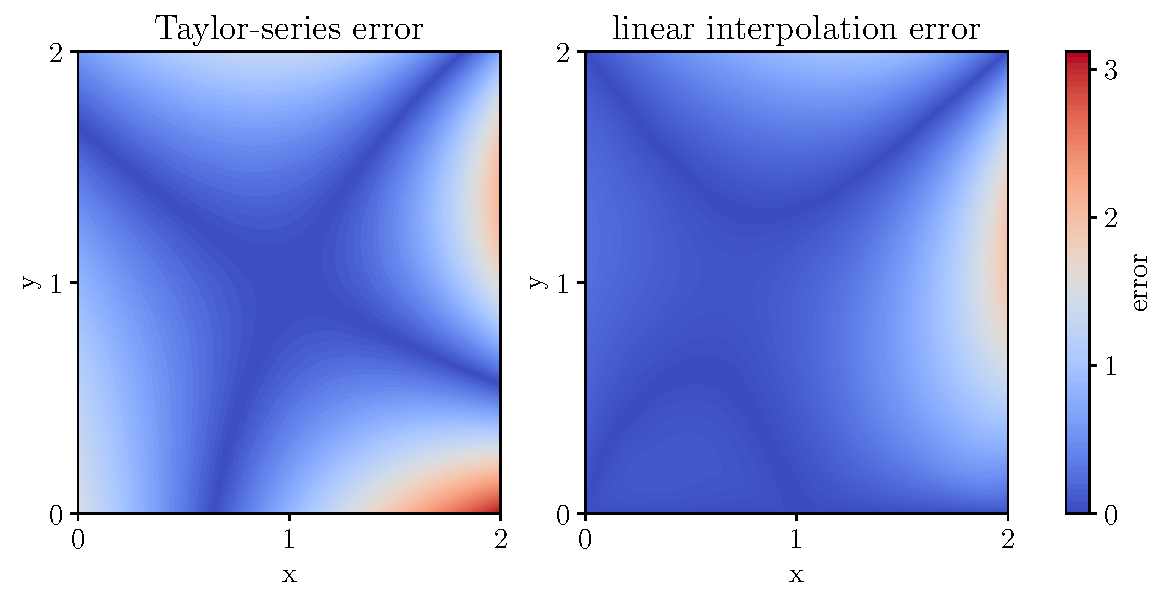
\includegraphics[width=0.9\linewidth]{bundles/interp_fig.pdf}
    \caption{A comparison of the accuracy of a first-order Taylor series taken about $(x,y)=(1,1)$ with linear interpolation of the four corner points on the function $f(x,y) = \sin(x)e^{y}$. While the errors are comparable between these two approximations, the patterns of these errors are notably different. This is because approximation by linear interpolation results in an affine model that can be different than the first-order Taylor series.}
    \label{fig:btb:interp}
\end{figure}
% \begin{align}
%     W_z &= \begin{bmatrix}
%         z_1 & z_2 & \cdots & z_M
%     \end{bmatrix}
% \end{align}


% \plan{
% \begin{itemize}
%     \item here is a nonlinear function, we can linearize this with a taylor series 
%     \item or, we can compute some samples of this function and linear interpolate between them 
%     \item for a linear function, this is exact (as is the first order taylor series) 
% \end{itemize}
% }

% \subsection{Trajectory Optimization}
% \plan{
% \begin{itemize}
%     \item trajectory optimization problems look like this:
%     \item one method for solving these problems is multiple shooting
% \end{itemize}
% }


\subsection{Approximation for Optimization}
We will now consider a general nonlinear optimization problem and examine how these linearization techniques can be utilized to form a convex approximation of the original problem. This approach is used in sequential convex programming (SCP) methods where nonconvex optimization problems are solved by iteratively approximating the problem as convex in the neighborhood of the local iterate and solving for a step direction \cite{gill2005, nocedal2006, malyuta2021, pantoja1989}. 

To demonstrate how an SCP method would work with the two approximation techniques outlined, we examine a generic constrained optimization of the following form:
% Given a primal variable $z \in \R{n_z}$, we consider equality-constrained problems of the following form:
%
\begin{mini}
    {z}{ \| r(z) \|_2^2 }{\label{btb:gen_nl_opt}}{}
    \addConstraint{c(z)}{=0,}{}
\end{mini}
%
with a decision variable $z \in \R{n_z}$, residual cost function $r : \R{n_z} \rightarrow \R{n_r}$, and constraint function $c : \R{n_z} \rightarrow \R{n_c}$. By approximating both of these functions as affine with a first-order Taylor series around a current iterate $\bar{z}$, we are left with the following convex optimization problem:
\begin{mini}
    {z}{ \| \hat{r}\|_2^2 }{\label{btb:lin_prob}}{}
    \addConstraint{\hat{r}}{= r(\bar{z}) + \frac{\partial r}{\partial z}(z - \bar{z})}{}
    \addConstraint{\hat{c}}{= c(\bar{z}) + \frac{\partial c}{\partial z}(z - \bar{z})=0}{}
    % \addConstraint{\hat{c}}{=0.}{}
\end{mini}
While this problem is convex and we are guaranteed to find a globally optimal solution if one exists, we do not have a guarantee of feasibility. There are circumstances in which the linearization of the constraint function results in infeasible problems \cite{nocedal2006}. In order to guarantee that this problem is always feasible, many sequential convex programming methods convert the constraint into a penalty and reformulate \eqref{btb:lin_prob} with an always-feasible variant,
\begin{mini}
    {z}{ \| \hat{r} \|_2^2 + \phi(\hat{c}) }{\label{btb:lin_prob_slack}}{}
    \addConstraint{\hat{r}}{= r(\bar{z}) + \frac{\partial r}{\partial z}(z - \bar{z})}{}
    \addConstraint{\hat{c}}{= c(\bar{z}) + \frac{\partial c}{\partial z}(z - \bar{z}),}{}
\end{mini}
where $\phi : \R{n_c} \rightarrow \R{}_+$ is a nonnegative penalty that discourages constraint violations.
% Common choices for this penalty are $\phi(s) = \rho \|s\|_2^2$ and $\phi(s) = \rho \|s\|_1$, where $\rho \in \R{}_+$ can be adjusted to trade-off between lowering the cost and lowering the constraint violation.
No matter the structure of the cost and constraint functions, the convex optimization problem in \eqref{btb:lin_prob_slack} is guaranteed to always have a solution. 

Alternatively, a linear interpolant like that shown in \eqref{btb:blend1} can be used to approximate the cost and constraint functions. To do this, $m$ sample points centered around the current iterate $\bar{z}$ are used to evaluate the cost and constraint functions. These values are then horizontally concatenated into the following matrices:
% 
% and horizontally concatenated as columns of $W_z = [z_1 \, \, z_2 \,\,\cdots\,\,z_m]\in \R{n_z \times m}$, and the cost and constraint functions are calculated for each of these samples and stacked in an analogous manner for $W_r = [r(z_1) \, \, r(z_2) \,\,\cdots\,\,r(z_m)]\in \R{n_r \times m}$ and $W_c = [c(z_1) \, \, c(z_2) \,\,\cdots\,\,c(z_m)]\in \R{n_c \times m}$. 
% 
\begin{align}
    W_z &= \begin{bmatrix}
        z_1 & z_2 & \cdots & z_m
    \end{bmatrix} \in \R{n_z \times m}, \label{btb:Wz}\\
    W_r &= \begin{bmatrix}
        r(z_1) & r(z_2) & \cdots & r(z_m)
    \end{bmatrix} \in \R{n_r \times m}, \label{btb:Wr}\\
    W_c &= \begin{bmatrix}
        c(z_1) & c(z_2) & \cdots & c(z_m)
    \end{bmatrix} \in \R{n_c \times m}.\label{btb:Wc}
\end{align}
The interpolation vector $\alpha \in \R{m}$ is used to interpolate between these samples and their corresponding cost and constraint values. These approximations are used to recreate the relaxed problem shown in \eqref{btb:lin_prob_slack} as the following:
% \begin{mini*}
%     {\alpha, s}{ \| W_r \alpha  \|_2^2 + \phi(s) }{\label{qp_standard_form2}}{}
%     \addConstraint{W_c \alpha }{=s,}{}
%     \addConstraint{\sum \alpha }{=1,}{}
%     \addConstraint{\alpha }{\geq 0,}{}
% \end{mini*}
\begin{mini}
    {\alpha}{ \| \hat{r} \|_2^2 + \phi(\hat{c}) }{\label{btb:lin_prob2}}{}
    % \addConstraint{\hat{z} }{=W_z \alpha}{}
    \addConstraint{\hat{r} }{=W_r \alpha}{}
    \addConstraint{\hat{c} }{=W_c \alpha}{}
    \addConstraint{\alpha}{\in \Delta^{m-1},}{}
\end{mini}
where the optimal solution is $z^* = W_z \alpha^*$.  It is important to note the similarities between \eqref{btb:lin_prob_slack} and \eqref{btb:lin_prob2}, where the only difference is the the method for approximating the cost residual and constraint functions. Another key difference between these methods is the implicit trust region present in the simplex constraint on $\alpha$. Since $\alpha \in \Delta ^{m-1}$, this means that the approximated functions are constrained to be within the convex hull of the sampled points. By utilizing a sampling scheme that only samples points within a set trust region, the solution to \eqref{btb:lin_prob2} is guaranteed to stay within the trust region.

% Here we have shown how to take a constrained nonconvex optimization problem and approximate it locally with a convex one, all without taking any derivatives. 
% \plan{
% \begin{itemize}
%     \item here is an arbitrary constrained optimization problem 
%     \item we can solve this by linearly interpolating
% \end{itemize}
% }


\section{The Trajectory Bundle Method}
% Modern optimal control is based on the formation and solving of trajectory optimization problems with potentially non-linear c.
In this section we outline a canonical trajectory optimization problem specification and use linearly interpolated trajectory bundles to approximate the cost and constraint functions. This formulation is not only general enough to handle a variety of robotics platforms, it can also be extended to solve batch state estimation problems that share the trajectory optimization problem structure.

Trajectories will be represented in discrete-time as a list of vectors. For a dynamical system with a state $x \in \R{n_x}$ and control $u\in\R{n_u}$, the discrete-time dynamics function $x_{k+1} = f(x_k, u_k)$ maps the state and control at time-step $k$ to the state at $k+1$. A trajectory comprised of $N$ time-steps is represented with $(x_{1:N}, \, u_{1:N-1})$, such that numerical optimization can be used to solve for these values. 

\subsection{Trajectory Optimization}
Trajectory optimization is a powerful tool for reasoning about challenging control problems by solving for the optimal control sequence with numerical optimization. This technique leverages advances in nonlinear programming to solve a variety of underactuated control tasks with nonlinear dynamics.  A canonical trajectory optimization problem considering a trajectory with $N$ time-steps is represented as the following:
%
\begin{mini}
    {x_{1:N}, u_{1:N-1}}{  \|r_N(x_N)\|_2^2 + \sum_{k=1}^{N-1}\|r_k(x_k,u_k)\|_2^2}{\label{btb:trajopt}}{}
    \addConstraint{x_{k+1}}{=f(x_k, u_k)}{}%{\quad \quad  k \in [1, N-1]}
    % \addConstraint{x_{1}}{=x_\text{ic},}{}
    % \addConstraint{x_{N}}{=x_\text{goal},}{}
    \addConstraint{c(x_{k}, u_k)}{\geq 0,}%{}{ \quad \quad k \in [1, N]}
\end{mini}
where $c(x_k)$ is a generic constraint function. We will assume that all relevant constraints will be expressed in this form, including initial/goal constraints, state/control limits, and other arbitrary constraints present in the problem. 

The problem format in \eqref{btb:trajopt} is often referred to as multiple shooting \cite{hargraves1987, betts2001}, where both the state and control histories are optimized over, and the trajectory only becomes dynamically feasible at constraint convergence. This differs from single shooting, where only the controls are optimized over, and a rollout is performed to recover the states. One important distinction between these two methods is that in single shooting, the discrete-time dynamics must be evaluated sequentially $N-1$ times during the rollout, where in multiple shooting, the $N-1$ dynamics constraints can be evaluated entirely in parallel. This is especially relevant with GPU-based physics simulation, where the speed of a single simulation can be comparable to thousands of simulations run in parallel. 

\subsubsection{Solving Multiple Shooting with Trajectory Bundles}
The trajectory bundle method is able to reason about the trajectory optimization problem in \eqref{btb:trajopt} without having to differentiate any of the cost, dynamics, or constraint functions. Instead of using derivatives to approximate these functions with their first-order Taylor series, sampled trajectories near the current iterate are used to evaluate these functions for approximation with linear interpolation. This idea shown in \ref{btb:sect:interp}
Given an initial guess or current iterate $(\bar{x}_{1:N}, \bar{u}_{1:N-1})$, the costs, constraint, and dynamics functions are computed for each of the $M$ samples surrounding each knot points. To demonstrate this, let us examine a single knot point, $k$, where the current iterate is $(\bar{x}_k, \bar{u}_k)$. From here, $m$ points are sampled near the iterate, and these samples are horizontally concatenated into the following matrices:
\begin{align}
    W_x^{(k)} &= \begin{bmatrix}
        x_{k,1} & x_{k,2} & \cdots & x_{k,m}
    \end{bmatrix} \in \R{n_x \times m}, \label{btb:Wx}\\
    W_u^{(k)} &= \begin{bmatrix}
        u_{k,1} & u_{k,2} & \cdots & u_{k,m}
    \end{bmatrix} \in \R{n_u \times m}, \label{btb:Wu}
    % W_r &= \begin{bmatrix}
    %     r(z_1) & r(z_2) & \cdots & r(z_m)
    % \end{bmatrix} \in \R{n_r \times m}, \label{btb:Wr}\\
    % W_c &= \begin{bmatrix}
    %     c(z_1) & c(z_2) & \cdots & c(z_m)
    % \end{bmatrix} \in \R{n_c \times m}.\label{btb:Wc}
\end{align}
after which, all of the cost, dynamics, and constraint functions are computed and stored in a similar fashion,
\begin{align}
    W_r^{(k)} &= \begin{bmatrix}
        r(x_{k,1}, u_{k,1}) & r(x_{k,2}, u_{k,2}) & \cdots & r(x_{k,m}, u_{k,m})
    \end{bmatrix} \in \R{n_r \times m}, \label{btb:Wr2}\\
    W_f^{(k)} &= \begin{bmatrix}
        f(x_{k,1}, u_{k,1}) & f(x_{k,2}, u_{k,2}) & \cdots & f(x_{k,m}, u_{k,m})
    \end{bmatrix} \in \R{n_x \times m}, \label{btb:Wf2}\\
    W_c^{(k)} &= \begin{bmatrix}
        c(x_{k,1}, u_{k,1}) & c(x_{k,2}, u_{k,2}) & \cdots & c(x_{k,m}, u_{k,m})
    \end{bmatrix} \in \R{n_c \times m}. \label{btb:Wc2}
\end{align}
These matrices are computed for time-steps $1\rightarrow N$, with time-step $N$ omitting the dynamics evaluation matrix $W_f$ (since there is no need to propagate dynamics after the end of the trajectory). Together, these matrices can be used to locally approximate the potentially nonconvex optimization problem in \eqref{btb:trajopt}  as the following convex optimization problem:
% x_{1:N}, u_{1:N-1}, \hat{c}_{1:N-1}, s_{1:N+1}, w_{1:N-1}
\begin{mini}
    {\alpha_{1:N}}{ \|W_r^{(N)} \alpha^{(N)} \|_2^2 + \sum_{k=1}^{N-1} \|W_r^{(k)} \alpha^{(k)}\|_2^2 + \phi(s) + \phi(w)}{\label{btb:trajopt_bundled}}{}
    \addConstraint{x_k}{=W_x^{(k)} \alpha^{(k)}}{}
    \addConstraint{u_k}{=W_u^{(k)} \alpha^{(k)}}{}
    \addConstraint{c_k}{=W_c^{(k)} \alpha^{(k)}}{}
    \addConstraint{x_{k+1}}{=W_f^{(k)} \alpha^{(k)} + s_{k+1}}{}
    \addConstraint{c_k + w_k}{\geq 0}{}
    % \addConstraint{\sum \alpha^{(k)} }{=1}{}
    % \addConstraint{\alpha^{(k)} }{\geq 0}{}
    \addConstraint{\alpha^{(k)}}{\in \Delta^{m-1}.}{}
\end{mini}
After each time this problem is solved, the new iterates $(x_{1:N}, u_{1:N-1})$ are used to generate $m$ new samples around the iterate, and the problem is formed and solved again. This is a sequential convex programming algorithm, where the solution to the original nonconvex optimization problem is solved for with a sequence of convex ones \cite{nocedal2006}.  In this implementation, the penalty function used is $\phi(\cdot) = \rho \|\cdot \|_1$ with a large ($\rho \in [10^5,10^8]$). As soon as the solver is able to treat the constraints as real constraints instead of penalties, the penalties are removed and true constraint satisfaction is achieved. 


\subsection{Batch State Estimation}
Another valuable extension of the trajectory bundle method is for batch state estimation, where the maximum a posteriori (MAP) can be solved for in a framework compatible with \eqref{btb:trajopt}. Like the Unscented Kalman Filter (UKF), this approach does not require any derivatives from the dynamics or measurement functions. 

We consider a dynamical system with the following process and measurement models:
\begin{align}
    x_{k+1} &= f(x_k )+ q_k, & q &\sim \mathcal{N}(0, Q), \label{btb:vanilla_kf_1}\\ 
    v_{k} &= g(x_{k}) + r_k, & r&\sim \mathcal{N}(0, R),\label{btb:vanilla_kf_2}
\end{align}
where $f : \R{n_x} \rightarrow \R{n_x}$ is the dynamics function, and $g : \R{n_x} \rightarrow \R{n_v}$ is the measurement function. Oftentimes there exists a Gaussian prior belief state, that is represented with $x_1 \sim \mathcal{N}(\mu_{ic}, \Sigma_{ic})$, representing the belief over the state estimate at the first time-step. From here, the MAP problem solving for the optimal mean $(\mu_{1:N})$ takes the form of the following optimization problem:
\begin{mini}
    {\mu_{1:N}}{  \|\mu_{ic} - \mu_1 \|^2_{\Sigma^{-1}} + \sum_{k=1}^{N-1} \|q_k\|_{Q^{-1}}^2 + \|r_{k+1}\|_{R^{-1}}^2}{\label{btb:map}}{}
    \addConstraint{\mu_{k+1}}{=f(\mu_k) + q_k}{}
    \addConstraint{y_{k}}{=g(\mu_k) + r_k,}{}
\end{mini}
which falls within the structure of the canonical trajectory optimization problem shown in \eqref{btb:trajopt}. The trajectory bundle method is then used to approximate the dynamics and measurement functions with $m$ samples at each time-step in the same way shown in \eqref{btb:Wx}-\eqref{btb:Wc2}


\begin{mini}
    {\mu_{1:N}}{   \|\mu_{ic} - \mu_1 \|^2_{\Sigma^{-1}} + \sum_{k=1}^{N-1} \|q_k\|_{Q^{-1}}^2 + \|r_{k+1}\|_{R^{-1}}^2}{\label{btb:map_bundle}}{}
    % \addConstraint{\mu_{k+1}}{=f(\mu_k) + q_k,}{\quad \quad k = 0,\ldots,m-1}
    % \addConstraint{y_{k}}{=g(\mu_k) + r_k,}{\quad \quad k = 1,\ldots,m}
    \addConstraint{\mu_k}{=W^{(k)}_{\mu}\alpha^{(k)}}{}
    \addConstraint{\mu_{k+1}}{=W^{(k)}_{f}\alpha^{(k)} + q_k}{}
    \addConstraint{v_{k}}{=W^{(k)}_{g}\alpha^{(k)} + r_k}{}
    \addConstraint{\alpha^{(k)}}{\in \Delta^{m-1},}{}
    % \addConstraint{\alpha^{(k)}}{\geq0,}{\quad \quad k = 1,\ldots,N}
\end{mini}
where $v_k$ are the true measurements (not being optimized over).  Since there are no hard constraints in this formulation, there is no need for a penalty $\phi$ to reduce the constraint violations. Instead, the process for solving \eqref{btb:map} simply involves forming the bundles, solving \eqref{btb:map_bundle}, and repeating until convergence. 

%
%
%
\section{Examples}
%
%
%
\begin{figure}
    \centering
    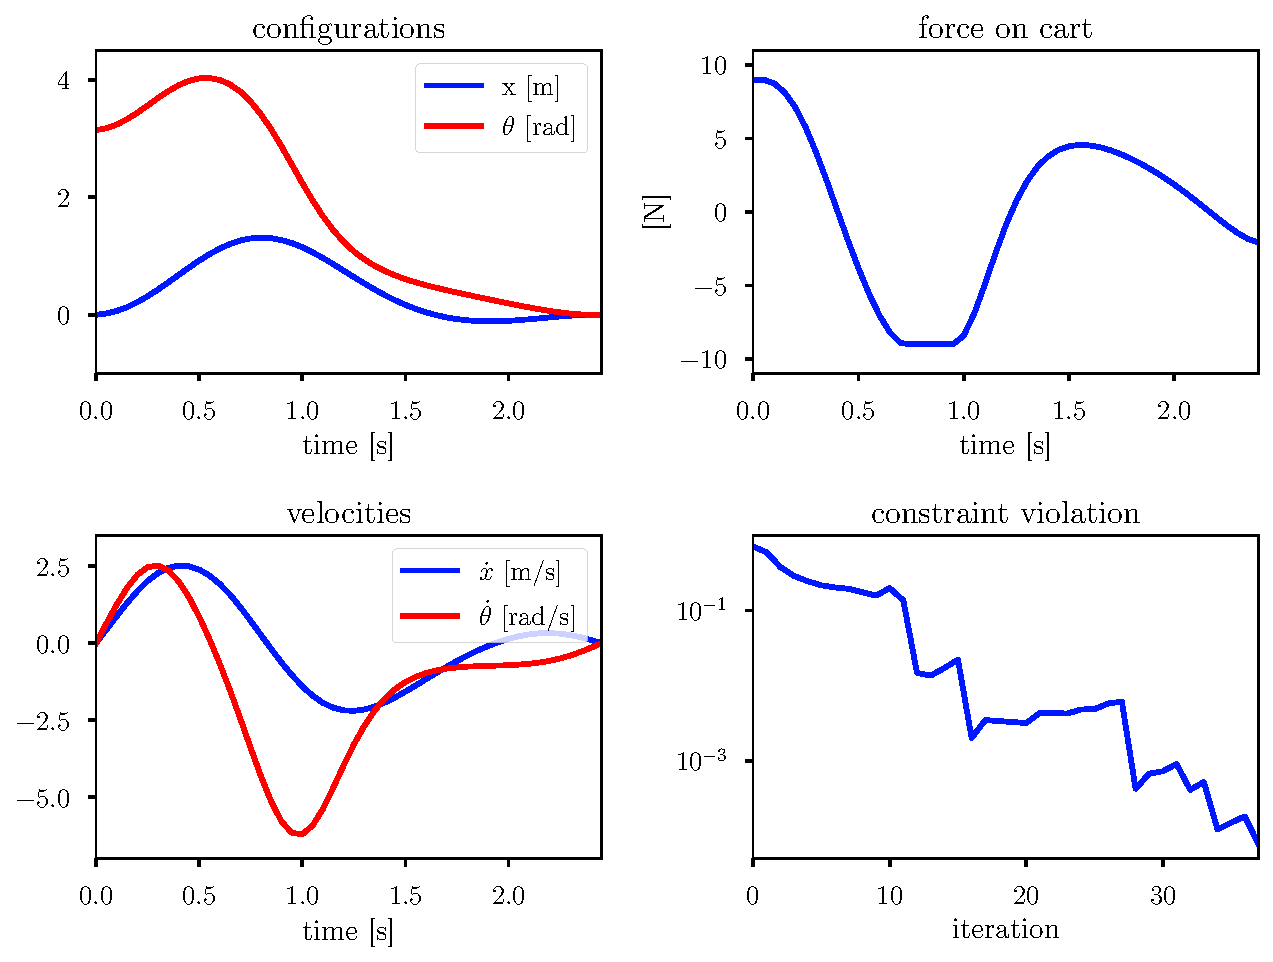
\includegraphics[width=0.9\linewidth]{bundles/examples/cartpole_fig.pdf}
    \caption{The classic cartpole swingup task solved with the trajectory bundle method. In 2.5 seconds, the pole must swing from the lowest position to the highest position, with control constraints on the force on the cart. Without the need for any derivatives, the proposed method is able to achieve tight constraint satisfaction in fewer than 40 iterations.}
    \label{fig:btb:cartpole}
\end{figure}

To demonstrate the efficacy of the trajectory bundle method for solving derivative-free nonconvex trajectory optimization problems, a variety of classic and challenging robotics problems are solved. In each of these examples, the discrete-time dynamics were evaluated with MuJoCo XLA (MJX) \cite{todorov2012}, such that the evaluation of the bundles is parallelized over both the samples for each time-step, as well as over all time-steps. The convex optimization problems are solved with Clarabel \cite{goulart2024} through CVXPY \cite{diamond}.

In the first example shown in Fig. \ref{fig:btb:cartpole}, a classic cartpole swingup is solved for using the trajectory bundle method. With a simple initialization where the configurations are linearly interpolated between the initial (pole down) and goal (pole up) states. From here, a 2.5 second trajector is solved for with input constraints on the force on the cart. The resulting solve takes fewer than 40 iterations with tight constraint satisfaction. 

\begin{figure}
    \centering
    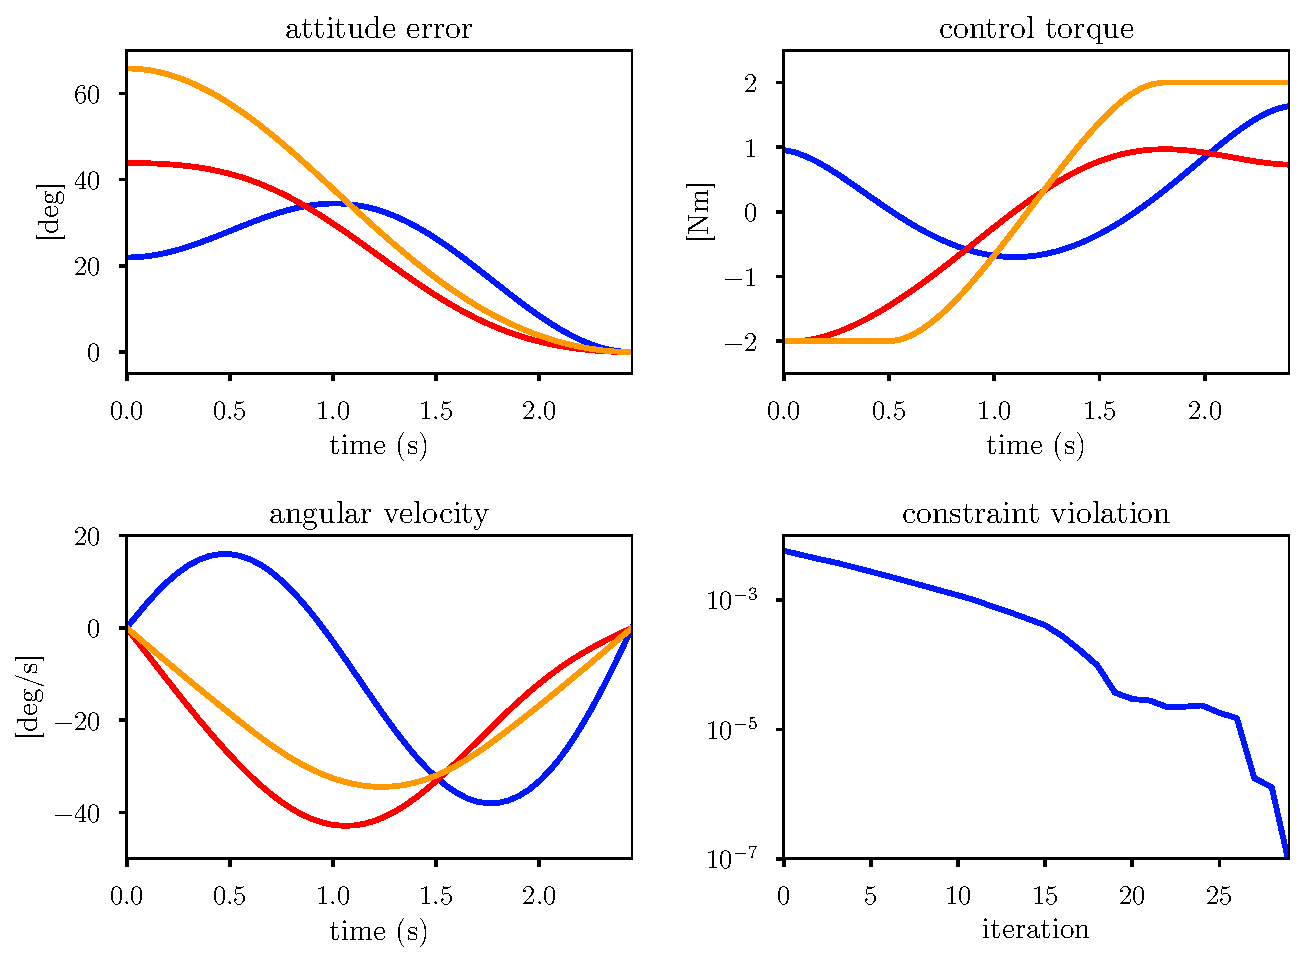
\includegraphics[width=0.9\linewidth]{bundles/examples/satellite_fig_2.pdf}
    \caption{A highly nonlinear satellite rest-to-rest slew is solved for with the trajectory bundle method. The satellite has direct torque control on the body with limits of 2 Nm.}
    \label{fig:btb:satellite}
\end{figure}


A more complex example is shown in \ref{fig:btb:satellite}, where a satellite is tasked with an aggressive rest-to-rest reorientation maneuver with limits on the control torque on the satellite. The trajectory bundle method is able to solve for an optimal trajectory in fewer than 30 iterations, with constraint satisfaction $<10^{-7}$. The resulting trajectory is aggressive and while it starts and stops with no angular velocity, it moves in excess of 50 degrees per second during the period with peak angular rates.

\begin{figure}
    \centering
    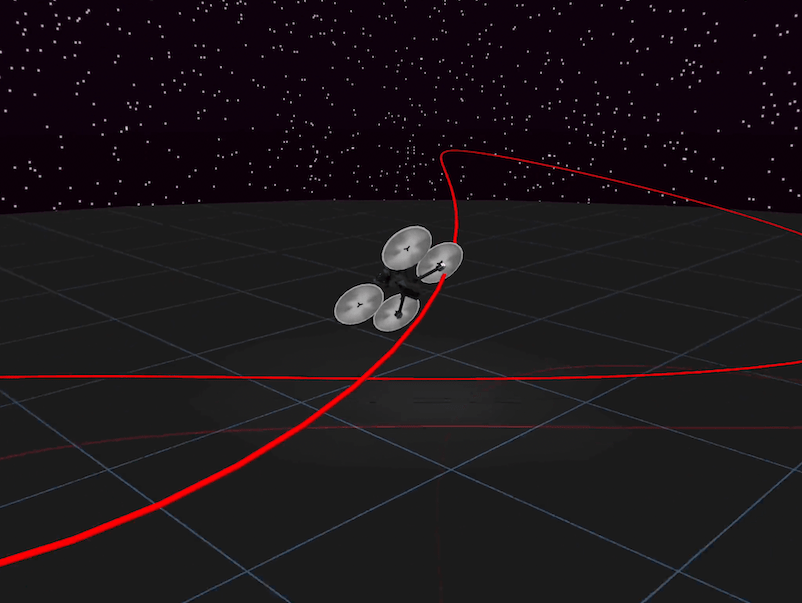
\includegraphics[width=0.5\linewidth]{bundles/examples/drone_shot.png}
    \caption{Given a figure eight reference trajectory, a quadrotor with rotor velocity control is tasked with tracking this trajectory as closely as possible.}
    \label{fig:btb:drone_shot}
\end{figure}


\begin{figure}
    \centering
    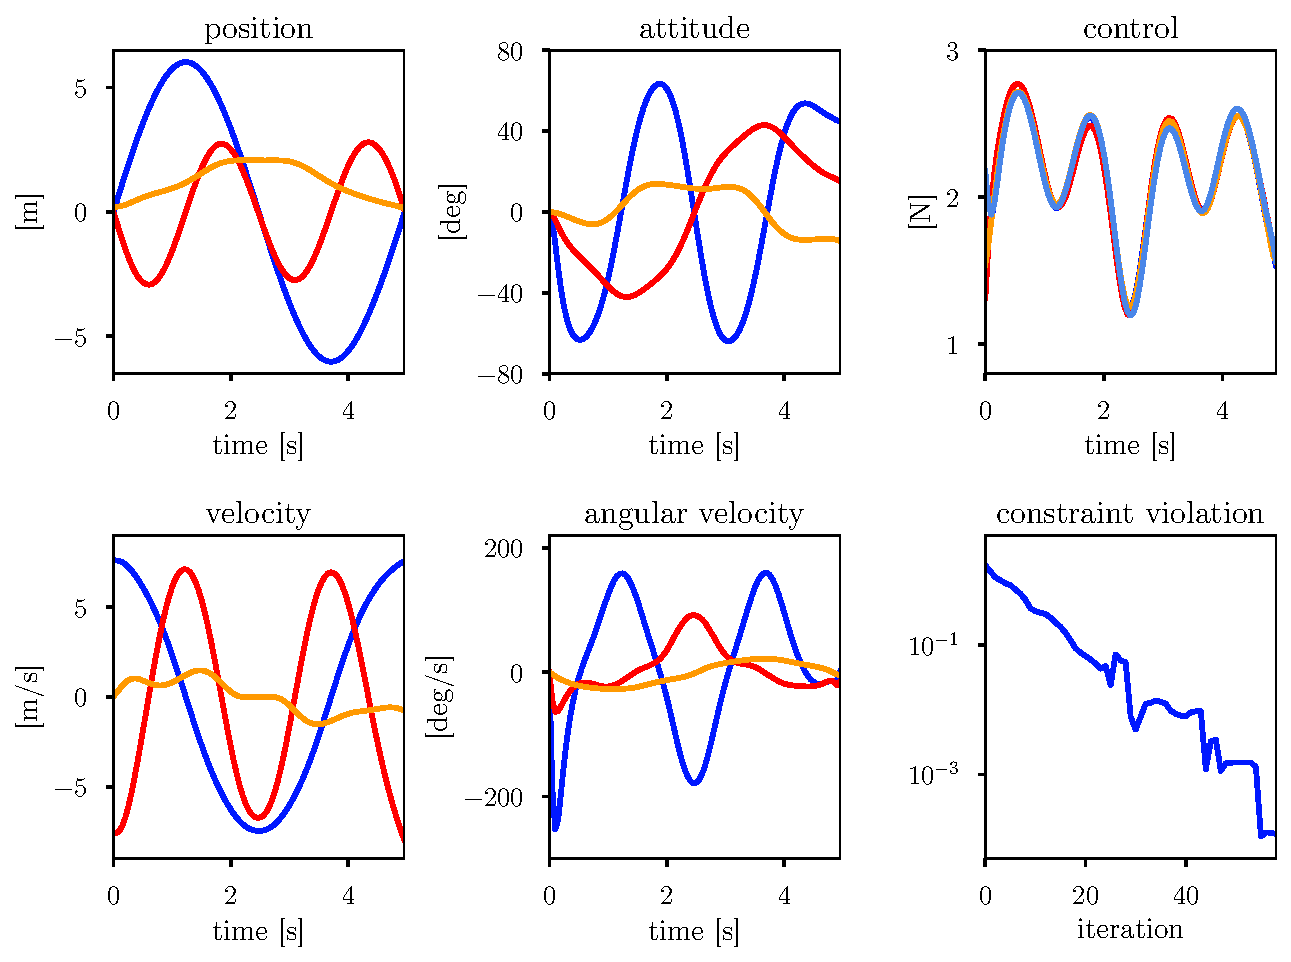
\includegraphics[width=0.9\linewidth]{bundles/examples/drone_fig.pdf}
    \caption{State and control convergence plots for the quadrotor tracking the skewed figure eight as shown in \ref{fig:btb:drone_shot}. The trajectory bundle method is used to solve for the aggressive trajectory, with angular velocity in excess of 200 degrees per second at times. The trajectory is discretized into 100 time-steps and the method converges to a solution in fewer than 60 iterations.}
    \label{fig:btb:drone}
\end{figure}


In Fig. \ref{fig:btb:drone_shot} and Fig. \ref{fig:btb:drone}, a quadrotor with rotor velocity control is tasked with tracking a skewed figure eight path through space. The trajectory is discretized into 100 knot points, and the resulting optimal trajectory smoothly tracks this aggressive reference while maintaining a smooth control commands. The angular velocity of the quadrotor is in excess of 200 degrees per second, resulting in highly nonlinear dynamics. In fewer than 60 iterations, the trajectory bundle method is able to solve this problem to the given constraint tolerance of $10^{-4}$. 


\begin{figure}
    \centering
    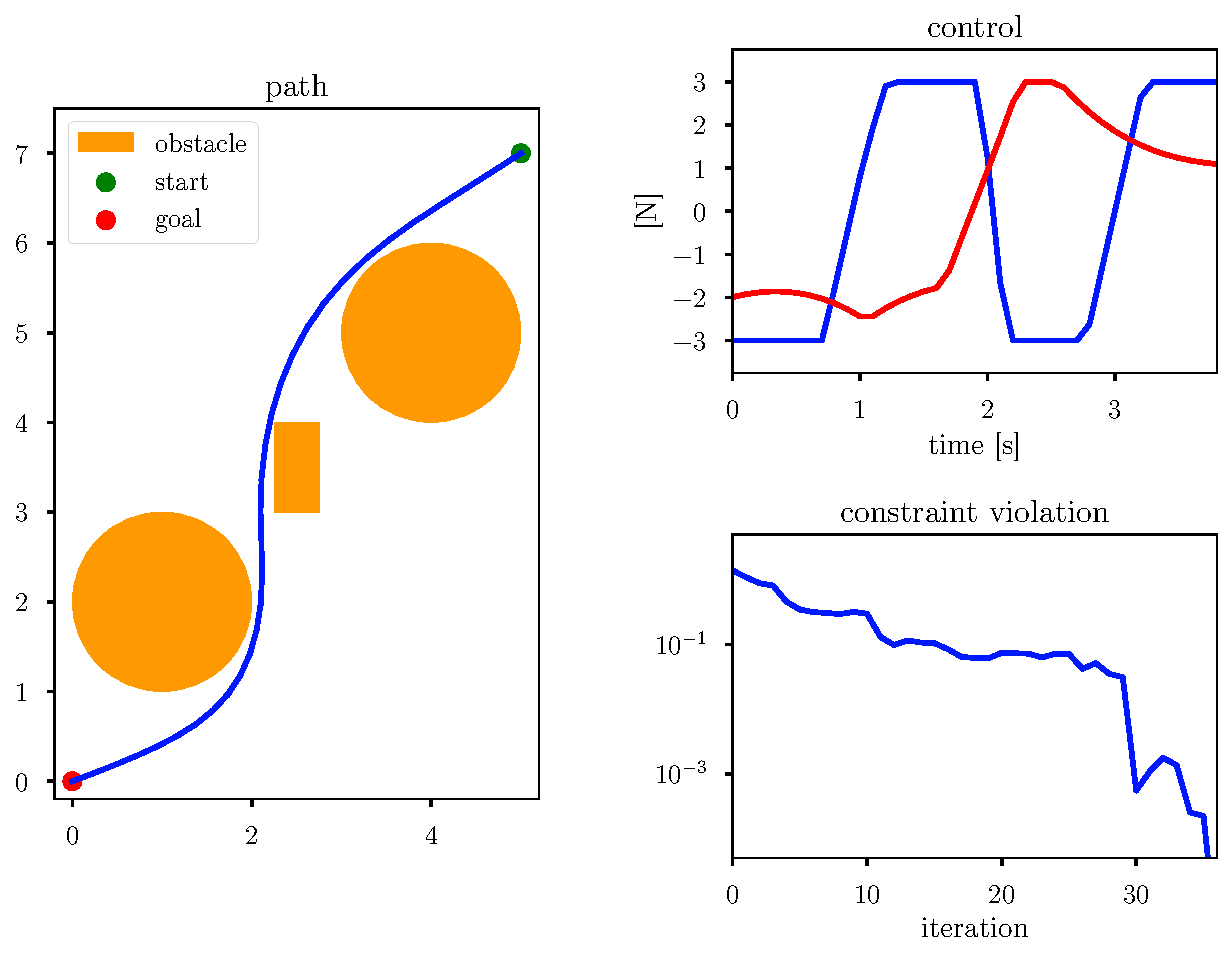
\includegraphics[width=0.9\linewidth]{bundles/examples/obstacle_fig.pdf}
    \caption{A double integrator with acceleration control is tasked with navigating around three obstacles to arrive at a goal position. The trajectory bundle method is able to directly reason about these arbitrary nonconvex constraints without the need for any derivatives, with strong constraint satisfaction and optimality achieved in fewer than 40 iterations.}
    \label{fig:btb:obstacle}
\end{figure}


To demonstrate the ability of the trajectory bundle method to handle arbitrary nonlinear constraints, a collision avoidance example is shown in Fig. \ref{fig:btb:obstacle}. In this example, the dynamics are that of a double integrator ($u = \ddot{x}$), and along with the three collision avoidance constraints, there is also a goal constraint at the origin. Without any derivative information from these nonconvex/nonlinear constraints, the trajectory bundle method is able to converge on a feasible collision-free trajectory in fewer than 40 iterations to a constraint satisfaction $<10^{-4}$.








\section{Conclusion}
In this work, we present the trajectory bundle method, a derivative-free trajectory optimization technique capable of solving nonconvex constrained optimization problems with strong constraint satisfaction. Instead of approximating the nonconvex functions with first-order Taylor series, the trajectory bundle method samples points locally and computes the cost, dynamics, and constraint functions for each of these samples in what we refer to as bundles. These bundles are used to linearly interpolate between these sampled values to approximate the cost, dynamics, and constraint functions. After the computation of these highly parallelizeable function calls, a convex optimization problem is solved where the nonconvex functions are replaced with linear interpolants, and the solution is used to generate new samples for the bundles.  The effectiveness of this method is demonstrated on a variety of robotics platforms.
%%% Local Variables:
%%% coding: utf-8
%%% mode: latex
%%% TeX-engine: xetex
%%% TeX-master: "../thesis"
%%% End: